
\chapter{面向云原生权限提升漏洞的智能化防控技术}\label{chap:method}


本章系统阐述面向云原生权限提升漏洞的智能化防控方法，先说明研究动机与方法框架，再介绍基本概念定义，并围绕知识库构建、多智能体策略生成与质量评估三项核心技术展开具体设计。

\section{研究动机}

本章讨论的问题，主要发生在漏洞已经披露但补丁尚未真正落地的处置阶段。对生产环境而言，第三方组件升级通常受到兼容性验证、变更审批与业务连续性要求等因素制约，补丁发布并不意味着系统能够立即完成修复。本文对 2020 至 2025 年间 55 个云原生权限提升漏洞的统计表明，$30.4\%$ 的漏洞因补丁延迟而长期处于可利用状态。与此同时，攻击者却可以借助公开公告、修复提交或社区讨论快速还原利用条件。因此，在补丁窗口期内形成临时防控措施，并尽快阻断关键利用条件、收敛攻击面和补足观测能力，已经成为云原生漏洞处置中的独立任务，而不只是正式修复前的附属动作。

\begin{figure}[htb]
    \centering
    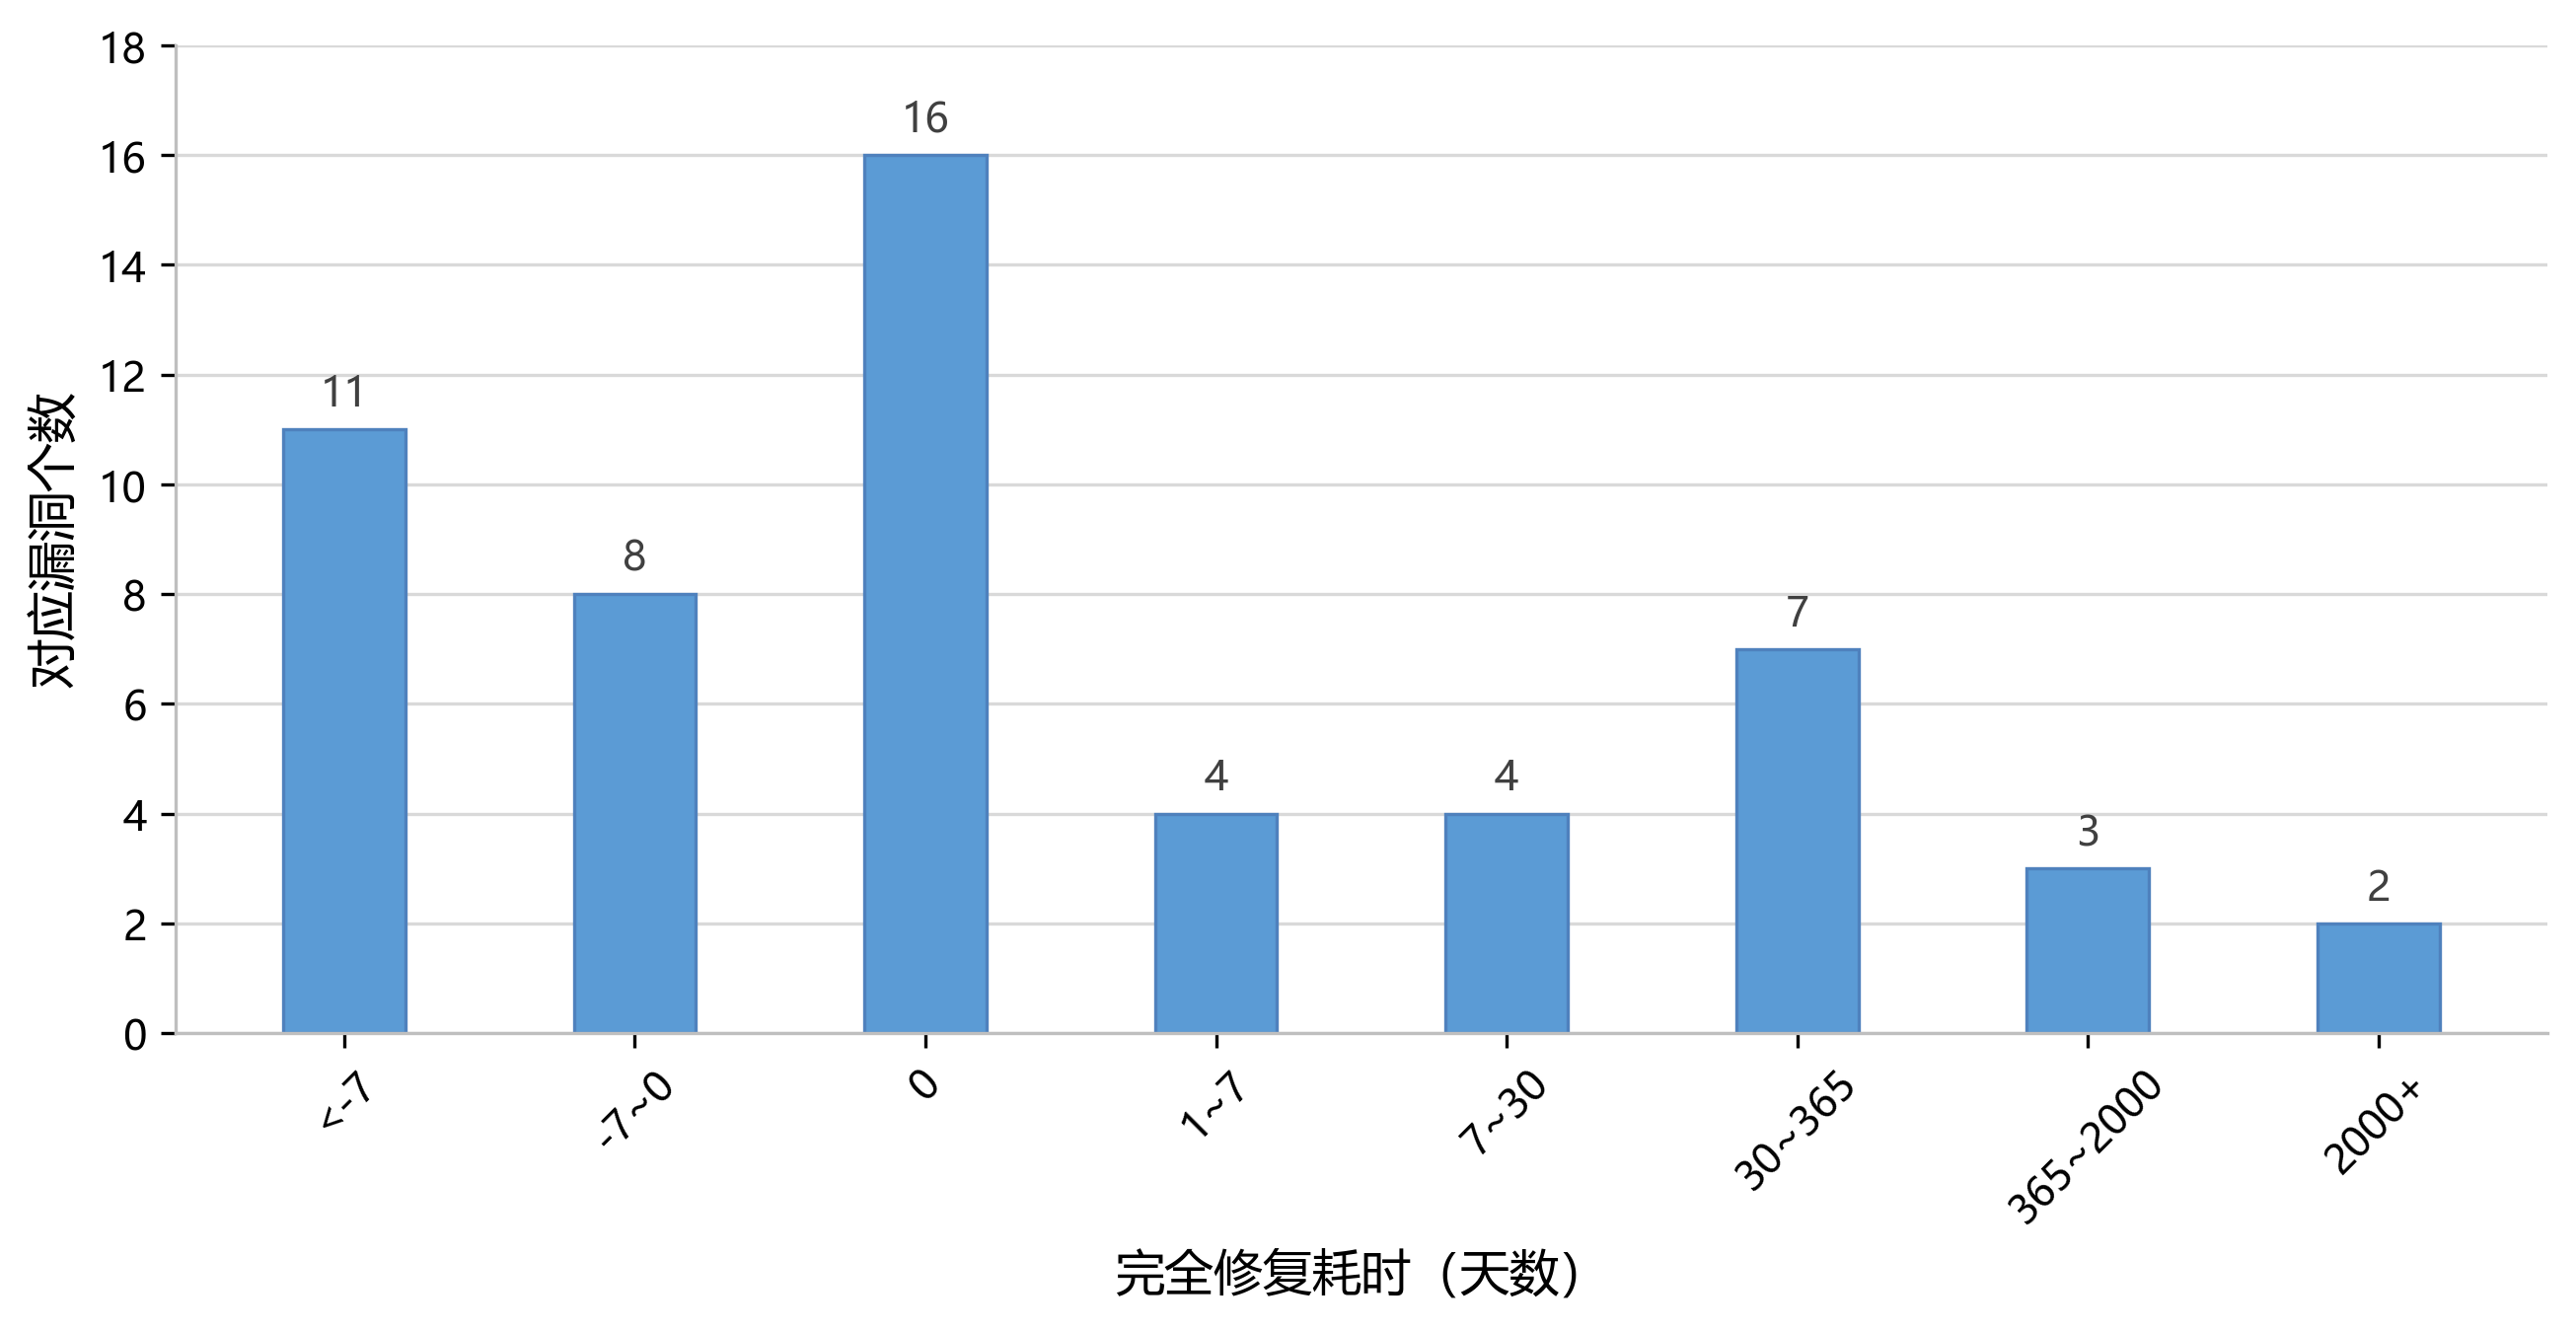
\includegraphics[width=0.8\textwidth]{images/cve-pub.png}
    \bicaption{云原生环境下权限提升漏洞的修复时间分布}{Distribution of remediation time for privilege escalation vulnerabilities in cloud-native environments}\label{fig:patch-window}
\end{figure}

这一处置任务的难点在于，临时防控策略并不能直接从 $\mathrm{CVE}$ 编号或简短公告中得到。权限提升漏洞往往同时涉及 $\mathrm{RBAC}$ 权限配置\cite{ferraiolo1995role}、控制平面交互、工作负载部署方式、运行时行为和网络可达关系等多个层面，并常与过度授权\cite{yang2023take}、授权检查缺陷、敏感信息泄露\cite{kubeguard_icws2025}等问题交织出现。真正有用的处置依据，通常分散在漏洞公告、修复提交、Issue/PR 讨论、配置清单与相关代码之中。要在较短时间内形成有效策略，需要先重建漏洞语义，再识别关键控制点，并据此判断应采用准入控制、$\mathrm{RBAC}$ 收敛、运行时监控还是网络隔离等措施。换言之，这里面对的不是单一规则编写问题，而是面向具体漏洞的证据组织与控制路径选择问题。

围绕云原生安全治理，现有工具已经覆盖了较完整的风险管控周期。静态层面，已有方法可对镜像依赖与 $\mathrm{Kubernetes}$ 清单进行扫描\cite{shamim2025prescription,k8smanifests2023}；动态层面，则包括基于 $\mathrm{eBPF}$ 的运行时观测与审计\cite{falco2025}、$\mathrm{OPA/Gatekeeper}$\cite{opa2025} 和 $\mathrm{Kyverno}$\cite{kyverno2025} 等准入控制机制，以及通过网络策略约束横向连通范围的防护手段\cite{Minna_2021,Budigiri_2021}。这些技术为集群安全提供了必要基础，但大多围绕通用基线核查和既有规则模式展开，更擅长识别普遍性风险；当目标转向某一具体漏洞时，它们往往缺少从多源证据出发、围绕利用条件组合控制措施的能力。实践中真正欠缺的，并不是新的单点工具，而是能够将已有工具与漏洞证据关联起来、面向补丁窗口期快速输出针对性临时策略的方法。

正是在这一点上，大语言模型提供了新的实现可能。其价值并不在于替代扫描器、准入控制器或运行时系统，而在于能够对异构文本与半结构化材料进行理解、归纳与重组，从中提取攻击语义、受影响对象与潜在控制点。如果将这种能力与现有安全工具的检测、约束和执行能力结合起来，便有机会形成一条从漏洞证据整理到策略生成、再到部署验证的协同处置路径。因此，本文的出发点并不是构造一种脱离现有生态的全新安全工具，而是探索如何将 $\mathrm{LLM}$ 与既有安全工具有效衔接，使其共同服务于补丁窗口期内的临时防控任务。

若要使这一思路真正落到可执行的方法设计上，还需要进一步回答以下三个问题。

\noindent\hangindent=1em\hangafter=1 (1) \textbf{如何构建面向具体漏洞的安全上下文}。权限提升漏洞的关键信息分散在代码仓库、漏洞公告、Issue/PR 讨论与修复提交等多类来源中。若缺乏统一的组织方式，模型很难准确把握漏洞成因、利用前提与影响边界。因此，方法首先需要建立可检索、可追溯的领域知识支撑，将分散证据转化为可供生成环节直接使用的安全上下文。

\noindent\hangindent=1em\hangafter=1 (2) \textbf{如何将漏洞语义映射为可部署的控制措施}。即便能够理解漏洞语义，临时防控策略的形成仍需要回答“在哪个控制面介入、采用何种约束方式、如何与现有工具配合”这一系列问题。也就是说，方法设计不仅要完成文本层面的归纳，还要把漏洞语义进一步转化为面向 Kubernetes 控制面的具体策略表达。

\noindent\hangindent=1em\hangafter=1 (3) \textbf{如何控制生成结果的不确定性}。大语言模型在将漏洞语义转化为策略代码时，仍可能出现幻觉、逻辑矛盾或偏离实际环境的问题。若缺乏有效的验证与校正机制，生成结果不仅可能无法阻断攻击，还可能干扰正常业务。因此，方法还必须考虑如何通过多阶段协同、结果评审与反馈优化，提高策略的有效性、无干扰性与可部署性。

基于上述动机，本文选择以多智能体协同方式组织整个防控流程，将证据整理、漏洞分析、策略生成、结果评审与反馈优化拆分为相互衔接的处理环节。这样的设计既服务于补丁窗口期内的快速响应需求，也为异构知识融合和生成结果控制提供了可操作的实现路径。后续内容将围绕这一思路，依次说明方法框架中的关键对象、知识支撑机制、协同生成流程以及质量控制方法。

\section{方法框架}

基于前文提出的现实需求，本文将补丁窗口期内云原生权限提升漏洞的防控问题建模为面向具体漏洞生成临时策略的自动化过程。按照控制手段的作用方式，相关措施可概括为监控策略与防护策略两个互补层次。其中，防护策略侧重在漏洞利用发生前阻断关键条件并收敛攻击面；监控策略侧重对运行时异常行为进行持续观测、告警与取证。围绕这两个目标，本文构建了基于多智能体安全策略管理的智能化漏洞防控框架。

\begin{figure}[htb]
    \centering
    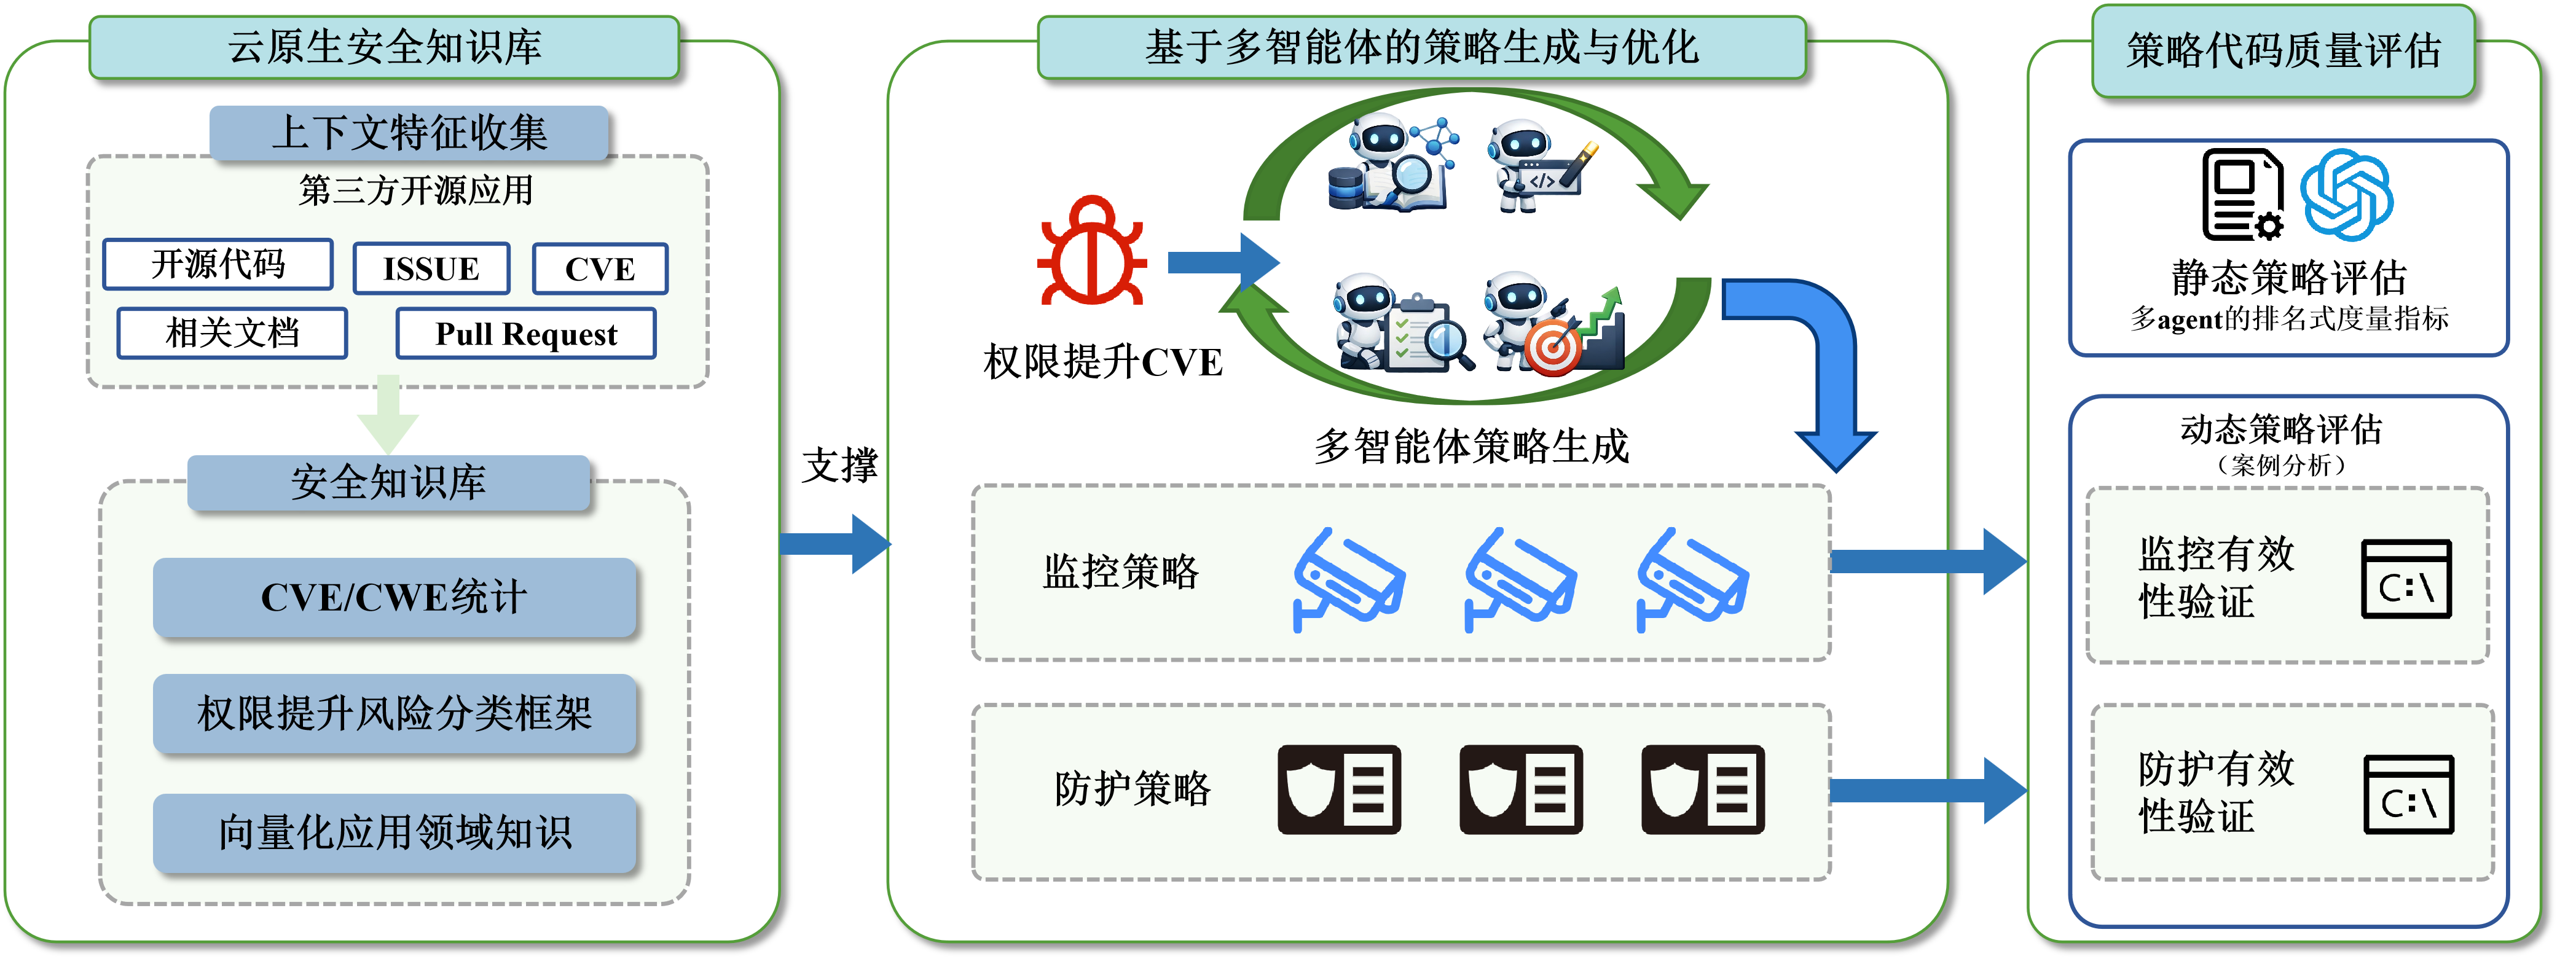
\includegraphics[width=1\textwidth]{images/总体框架.png}
    \bicaption{基于多智能体的策略化漏洞防控研究总体框架}{Overall multi-agent framework for strategy-based vulnerability prevention and control based on large language models}\label{fig:overall-framework}
\end{figure}

如图~\ref{fig:overall-framework}所示，该框架以权限提升类 $\mathrm{CVE}$ 为输入，依托大语言模型与多智能体协同，结合检索增强生成、思维链推理与反馈优化等技术，围绕安全知识支撑、策略生成、策略验证和平台工具建设，形成从漏洞披露到输出结构化 JSON 临时防控策略的自动化流程。具体而言，系统首先从代码仓库、漏洞公告、Issue/PR 讨论与补丁提交中提取多源证据，构建可追溯的漏洞安全知识库；随后通过安全知识、漏洞分析、策略生成、策略评审与策略优化等智能体协同，将漏洞语义转化为面向 Kubernetes 平台的监控与防护策略；最后结合质量评价与平台工具，实现结果排序、人工复核与部署验证。下面将依次对该流程涉及的对象定义、知识支撑机制、生成方法与评价过程展开说明。

\subsection{基本概念定义}

\subsubsection{基本对象} % 增加编号

为形式化描述面向漏洞的安全策略生成问题，本文将方法中的核心对象抽象为漏洞实例、安全上下文与安全策略三类实体。本文涉及的主要记号与核心术语已在前置部分的符号清单与术语表中汇总，这里仅给出与方法定义直接相关的形式化说明。记候选策略全集为 $\Pi$。策略质量评价所涉及的维度与记号将在下一小节中进一步给出。

\textbf{定义 1（漏洞实例）}。设 $\mathcal{V}$ 为漏洞实例空间。任一漏洞实例表示为
\[
v=\langle \mathit{id},\,d,\,m \rangle\in\mathcal{V}
\]
其中，$\mathit{id}$ 为漏洞标识符（如 CVE 编号），$d$ 为漏洞描述文本，$m$ 为与漏洞相关的元数据，用于刻画其严重性、受影响组件及版本范围等属性。

\textbf{定义 2（安全上下文）}。给定漏洞实例 $v$，其安全上下文 $c\in\mathcal{C}$ 定义为带来源标识的有限证据集合：
\[
c = \bigl\{\,\langle t_i,\,\mathit{src}_i \rangle \mid i\in[n_c] \,\bigr\}
\]
其中，$t_i$ 表示证据内容，$\mathit{src}_i$ 表示来源标识（如文档路径、公告链接或代码位置）。该定义强调上下文不仅提供与漏洞相关的背景事实，而且保留事实来源，以支撑后续策略生成与结果复核。

\textbf{定义 3（安全策略）}。针对给定漏洞实例 $v$ 的完整安全策略表示为三元组
\[
\pi = \langle \mathit{type},\;\mathit{method},\;\mathit{action} \rangle
\]
其中，$\mathit{type}\in\{\mathrm{mon},\mathrm{prot}\}$ 表示策略属于监控型还是防护型；$\mathit{method}=(m_1,\ldots,m_k)$ 表示控制机理序列，$\mathit{action}=(a_1,\ldots,a_k)$ 表示与之对应的执行表达序列。二者满足一一对应关系，即每个 $m_i$ 均对应一个可部署的 $a_i$，共同构成完整的防控措施单元。

对给定漏洞实例 $v$，生成阶段得到的候选策略集合记为 $\Pi_v\subseteq\Pi$。


\subsubsection{质量评价指标}

由于不同漏洞样本在业务环境、证据完备程度与候选策略规模上存在差异，若直接采用绝对分值，容易引入尺度漂移与比较偏置。与此同时，监控策略与防护策略在优化目标上并不完全同质，前者更强调观测、告警与取证能力，后者更强调阻断、收敛与约束效果。因此，本文在评价阶段先按策略类型划分候选集合，再在各自子集中实施基于排序的相对评价。记类型集合为 $\mathcal{T}=\{\mathrm{mon},\mathrm{prot}\}$，对任意 $\tau\in\mathcal{T}$，定义
\[
\Pi_v^{\tau}=\Pi_v\cap\Pi_{\tau}
\]
表示漏洞实例 $v$ 在类型 $\tau$ 下的同质候选子集。下文若不强调策略类型，统一用 $\Pi_v$ 表示漏洞实例 $v$ 的候选策略集合；当需要区分监控型与防护型时，再使用 $\Pi_v^{\tau}$ 表示对应子集。记评价维度集合为 $\Delta=\{E,I,D\}$，分别对应有效性、无干扰性与可部署性。

\textbf{定义 4（三维质量向量）}。策略质量由映射 $q\colon\Pi\to[0,1]^3$ 给出：
\[
q(\pi) = \bigl(E(\pi),\;I(\pi),\;D(\pi)\bigr)
\]
其中，$E$ 衡量策略对主要攻击路径与关键风险面的覆盖程度，$I$ 衡量策略对正常业务的扰动程度及误报风险，$D$ 衡量策略在现有环境中的落地难度与执行清晰度。

\subsection{云原生权限提升安全知识库}

如图~\ref{fig:cve-database}所示，本节围绕漏洞实例 $v$ 构建可追溯云原生权限提升安全知识库 $\mathcal{K}_v$，并通过检索形成安全上下文 $c$，为后续策略生成提供带来源标识的证据支撑。

\begin{figure}[htb]
    \centering
    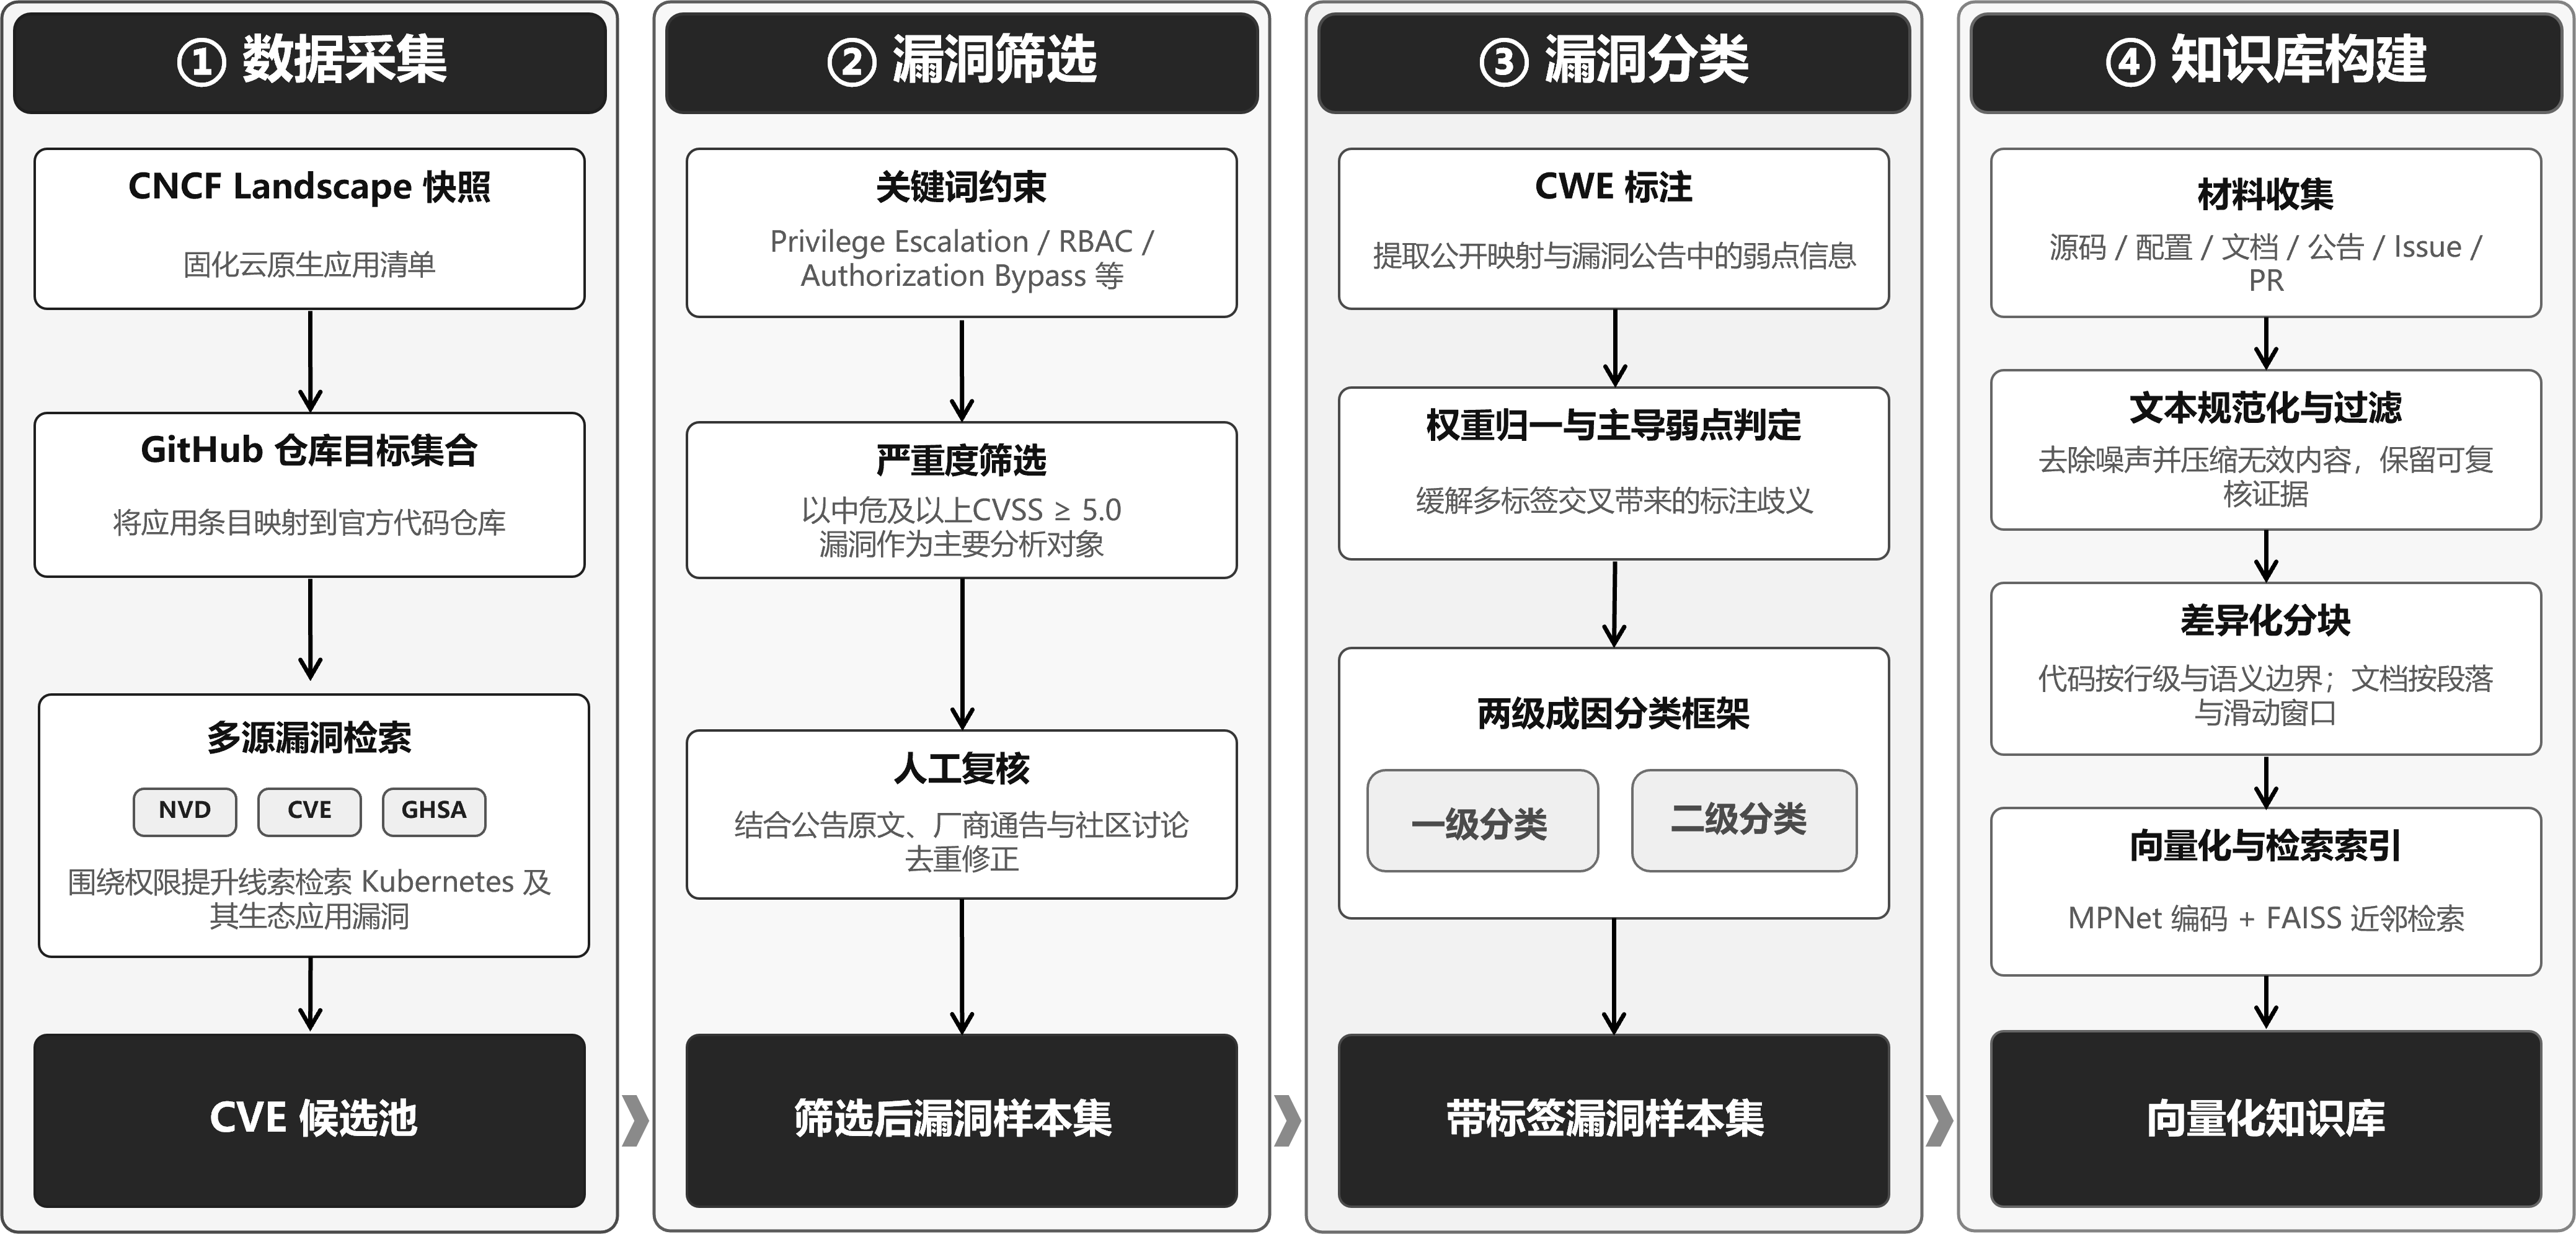
\includegraphics[width=0.92\textwidth]{images/chap3_cve_database.png}
    \bicaption{云原生权限提升漏洞知识库构建}{Overview of the cloud-native privilege escalation vulnerability knowledge base construction}\label{fig:cve-database}
\end{figure}


\subsubsection{数据采集}

本文以 Kubernetes 及其生态开源应用为研究对象，首先从 CNCF Landscape 获取云原生应用清单，并对清单进行快照固化，以保证采集过程可复现。随后，将清单条目名称映射到其官方代码仓库，形成后续漏洞检索与证据收集的目标集合。

在此基础上，本文综合使用 NIST NVD\footnote{NIST NVD（National Vulnerability Database）：\url{https://nvd.nist.gov/}}、MITRE CVE 官方库\footnote{MITRE CVE：\url{https://cve.mitre.org/}}与安全公告平台 GitHub Security Advisory\footnote{GitHub Security Advisory：\url{https://github.com/advisories}}三个来源，围绕权限提升线索对 Kubernetes 及其生态应用开展多源漏洞检索，获得初步 CVE 候选池。

\subsubsection{漏洞筛选}

为从 CVE 候选池中筛选出高质量样本，本文采用关键词约束、严重性阈值与人工复核相结合的三重过滤策略：
\begin{itemize}
    \item \textbf{关键词约束}：在 CVE 描述与参考链接中匹配 Privilege Escalation、Authorization Bypass、Improper Access Control、RBAC、ServiceAccount、ClusterRole、Container Escape/Sandbox Escape/Breakout 等关键词；
    \item \textbf{严重性阈值}：采用 CVSS v3.x 评分，并以 $\geq 5.0$ 的中危及以上漏洞为主要对象；
    \item \textbf{人工复核}：对候选条目结合公告原文、厂商通告与社区讨论进行复核，剔除重复或与权限提升无关的记录，并补全攻击前提、影响面与可用缓解信息。
\end{itemize}
最终保留的结构化字段包括 CVE 编号、漏洞摘要、披露时间、受影响组件与版本范围、修复版本、CVSS 评分、参考链接，以及与修复相关的补丁提交记录等。上述字段与漏洞实例 $v=\langle \mathit{id},\,d,\,m \rangle$ 直接对应：CVE 编号即标识符 $\mathit{id}$，漏洞摘要构成描述 $d$，其余属性如严重性评分、受影响版本和参考链接等共同构成元数据 $m$。

为保证数据构建过程可复现，本文对同一批次样本采用统一快照方式完成采集，并在构建配置中记录应用清单快照、检索时间窗口、纳入与剔除准则以及去重规则。对于来自不同数据源但指向同一漏洞事实的记录，以 CVE 编号为主键进行合并；对于无独立编号但经公告与补丁信息确认指向同一漏洞事件的记录，则视为重复项而不重复计数。

\subsubsection{漏洞分类}

漏洞样本的分类方式直接影响后续策略生成的针对性。为此，本文构建了面向策略生成场景的两级成因分类框架，旨在为模型提供稳定且可解释的风险语义线索，从而约束推理路径、辅助关键控制点与实施路径的选择，提升输出策略的可部署性、可验证性与副作用可控性。

首先，本文依据公开映射与公告信息提取每个 CVE 的 CWE（Common Weakness Enumeration）标签，并统计不同 CWE 的出现频次。CWE 是 MITRE 维护的软件弱点枚举体系，可用于将具体 CVE 归并到更抽象的弱点类型。

\begin{figure}[htb]
    \centering
    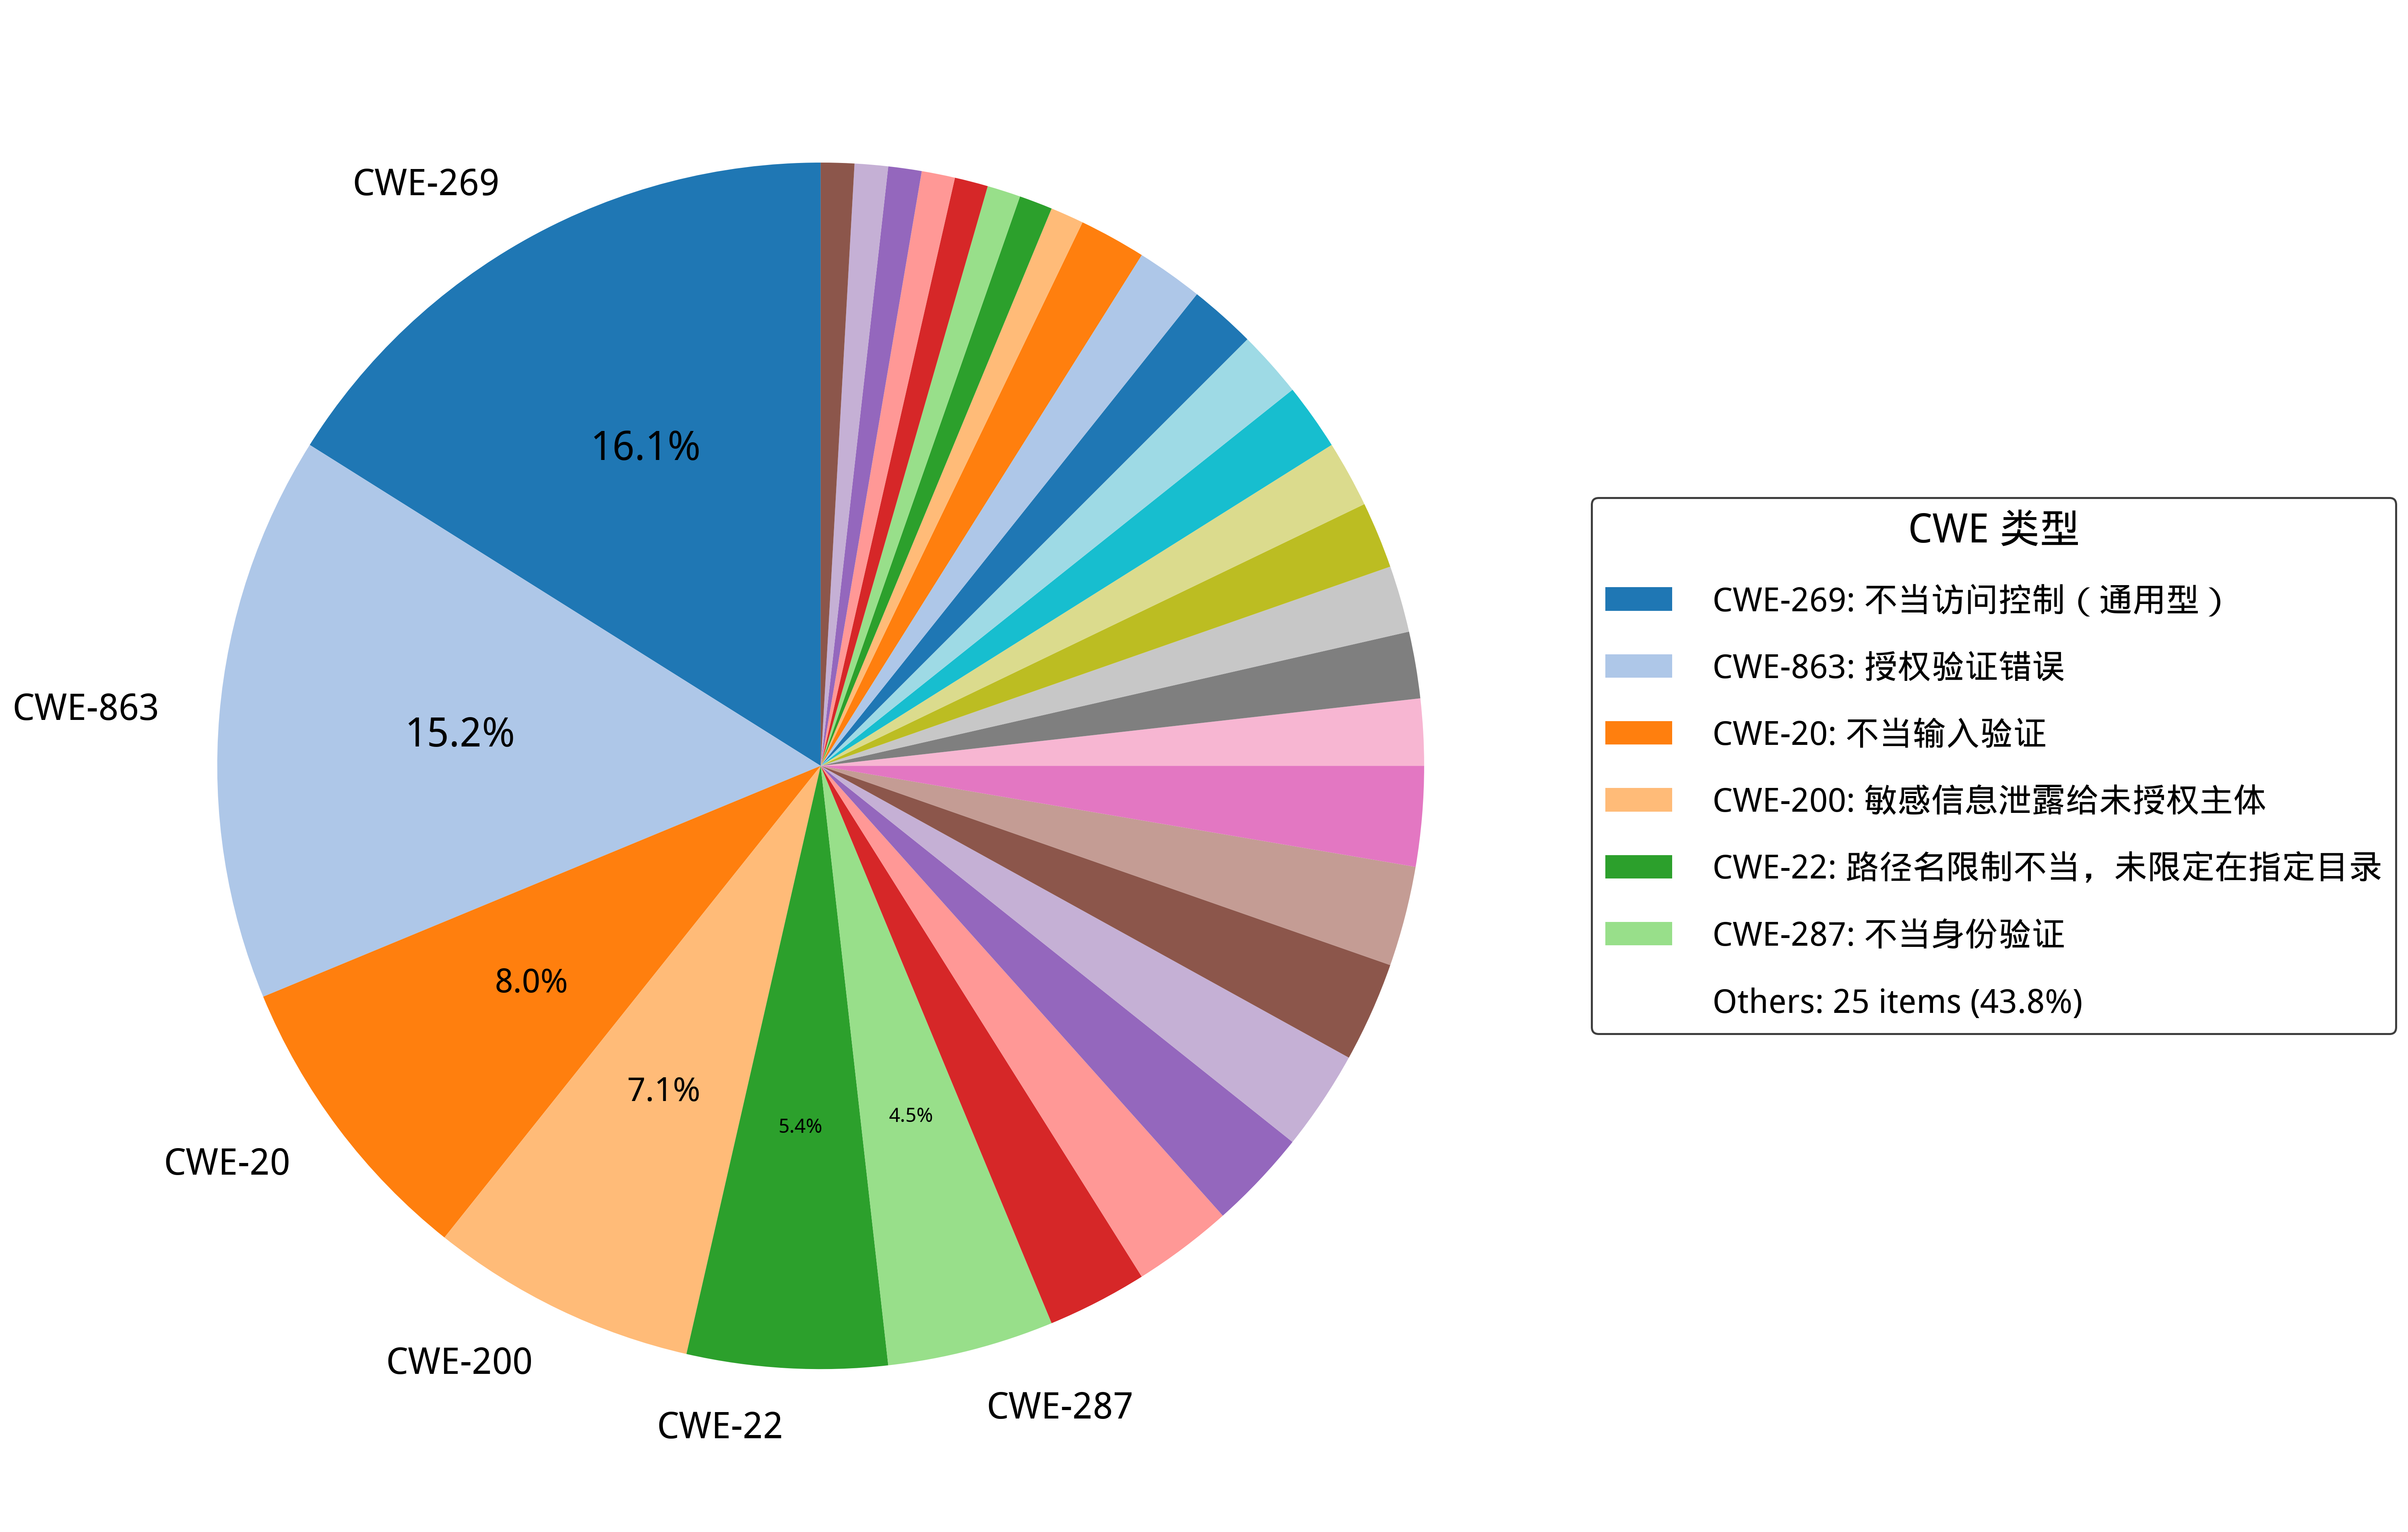
\includegraphics[width=1\textwidth]{images/cwe_distribution_pie.png}
    \bicaption{Kubernetes 权限提升 CVE 对应的 CWE 类型占比}{Distribution of CWE categories corresponding to Kubernetes privilege escalation CVEs}\label{fig:cwe-distribution-ch3}
\end{figure}

CWE 体系并不是严格互斥的分类框架。同一漏洞往往会同时对应多个弱点条目，不同条目在抽象层次上也可能彼此交叉。在本文收集的 55 个权限提升漏洞中，有 20 个样本同时关联两个及以上 CWE 标签，占比 36\%。为更客观地反映 CWE 分布，统计时令每个 CVE 的总权重为 1，多标签样本按标签数平均分配。结果表明，授权不当、权限管理不当等访问控制类弱点常与输入验证不当等问题同时出现，这说明权限提升漏洞通常具有复合成因。仅依赖单一 CWE 标签，难以为后续防控策略提供稳定的语义约束，因此有必要进一步构建面向防控动作的成因分类框架。

基于这一问题，本文进一步提出面向云原生权限提升漏洞的两级成因分类框架，并为每个漏洞确定一级类和二级类标签。一级分类用于概括高层风险来源，如安全逻辑缺陷、配置缺陷、代码注入和敏感信息泄露；二级分类则进一步细化到更贴近防控动作选择的类型，如授权验证不完善、默认不安全配置等。经过这样的整理，漏洞分析结果可以更自然地映射到 RBAC 最小权限、准入控制、网络隔离、运行时策略与审计等具体控制点。

在策略生成阶段，分类结果作为提示词中的结构化约束，引导模型先识别漏洞的主要成因，再定位关键控制点，最后组织可执行的防控动作，从而减少泛化建议和无关信息，提高策略的针对性与可部署性。完整的一级、二级分类及其与 CWE 的对应关系见附录表~\ref{tab:vuln-cwe-mapping}。

为降低多标签条件下的标注歧义，本文对每个样本只保留一个主导的一级类和二级类标签。判定时优先选择直接造成权限边界突破的成因；其余伴随弱点仍保留在 CWE 映射表中，作为补充语义信息。对于边界不清或存在多种解释路径的样本，再结合漏洞公告、修复补丁语义与攻击路径描述进行复核后裁决。

\begin{table}[htb]
    \centering\bicaption{云原生权限提升漏洞分类框架（CWE 对应详见附录表~\ref{tab:vuln-cwe-mapping}）}{Classification framework for cloud-native privilege escalation vulnerabilities (see Appendix Table~\ref{tab:vuln-cwe-mapping} for the CWE mapping)}\label{tab:cloud-native-vuln}
    \small
    \setlength{\tabcolsep}{3pt}
    \noindent\renewcommand{\arraystretch}{0.9}

    \begin{tabular}{ >{\centering\arraybackslash}p{3cm} >{\raggedright\arraybackslash}p{3cm} >{\raggedright\arraybackslash}p{3cm} }
        \toprule
        \textbf{一级分类} & \textbf{二级分类} & \textbf{示例 CVE} \\
        \midrule
        \multirow{2}{*}{配置缺陷} & 冗余权限 & \mbox{CVE{-}2023{-}30512} \\
         & 网络隔离不足 & \mbox{CVE{-}2020{-}4062} \\
        \midrule
        \multirow{4}{*}{安全逻辑缺陷} & 访问控制缺陷 & \mbox{CVE{-}2022{-}24768} \\
         & 身份验证绕过 & \mbox{CVE{-}2023{-}22482} \\
         & 输入验证不足 & \mbox{CVE{-}2023{-}3955} \\
         & 授权验证不完善 & \mbox{CVE{-}2022{-}21701} \\
        \midrule
        \multirow{3}{*}{敏感信息泄露} & API端口暴露 & \mbox{CVE{-}2022{-}1902} \\
         & 日志泄露 & \mbox{CVE{-}2019{-}10165} \\
         & 配置文件泄露 & \mbox{CVE{-}2019{-}3869} \\
        \midrule
        \multirow{2}{*}{代码注入} & 命令注入 & \mbox{CVE{-}2021{-}41254} \\
         & 路径遍历 & \mbox{CVE{-}2022{-}24877} \\
        \bottomrule
    \end{tabular}
\end{table}

以下对各一级分类分别展开说明。

\textbf{配置缺陷}指应用或基础设施的配置不当导致的安全漏洞，主要包括两种情形：
\begin{itemize}
    \item 过度权限配置：Kubernetes RBAC 配置不当、Role/ClusterRole 规则范围过宽或绑定关系不合理等，使低权限主体获得超出其职责的资源访问与高危操作能力。该类问题在第三方应用接入场景中尤为常见，并已被证明可被用于接管集群关键资源\cite{o1995redundant,yang2023take}。
    \item 网络隔离不足：容器、Pod或服务间缺乏网络隔离，导致攻击者可以横向移动获取其他权限。
\end{itemize}

\textbf{安全逻辑缺陷}指应用代码中的安全机制设计或实现不当，涵盖以下情形：
\begin{itemize}
    \item 访问控制缺陷：应用的权限检查不完全或存在逻辑漏洞，允许绕过权限验证；
    \item 身份验证绕过：认证机制设计缺陷，攻击者可以冒充他人身份或跳过认证步骤；
    \item 输入验证不足：对请求参数、资源标识或边界条件的校验不充分，导致攻击者借由异常输入扩大权限边界或触发越权路径；
    \item 授权验证不完善：权限检查在某些操作路径或边界条件下缺失。
\end{itemize}

\textbf{敏感信息泄露}指重要的身份、密钥或权限信息意外暴露，常见形式包括：
\begin{itemize}
    \item API 端口暴露：管理接口、内部 API 或调试端口未受保护暴露在网络上；
    \item 日志泄露：错误泄露的日志文件中包含密钥、命令历史等敏感信息；
    \item 配置文件泄露：配置文件包含硬编码的凭证或密钥。
\end{itemize}

\textbf{代码注入}指应用对用户输入的处理不当，使攻击者得以注入恶意代码，典型子类包括：
\begin{itemize}
    \item 命令注入：应用直接执行用户提供或可控的命令，攻击者可以执行任意系统命令；
    \item 路径遍历：应用文件访问检查不完整，攻击者可以访问系统其他部分的文件。
\end{itemize}

\subsubsection{知识库构建}

知识库构建阶段的目标是将与漏洞 $v$ 相关的多源材料组织为带来源标注的证据集合，并建立支持按需取证的检索能力。围绕 $v$ 构建知识库 $\mathcal{K}_v$ 后，策略生成阶段即可通过语义检索提取相关证据片段，并按需组装为安全上下文 $c$，为后续分析提供可追溯的事实依据。

具体而言，本文首先针对每个漏洞关联的开源应用仓库收集代码、配置与文档等可读文本，同时纳入与漏洞相关的安全公告、议题（Issue）/合并请求（Pull Request）讨论以及修复提交信息。随后，对文本进行最小化规范，并过滤超长或二进制内容，以降低噪声与资源开销。

在完成材料收集后，为兼顾证据粒度与可复核性，本文对不同材料采用差异化分块策略：对代码和配置按行切分，并尽量对齐函数或语义边界；对文档则按段落与窗口切分，并保留适当重叠，以减少跨块语义断裂。

在此基础上，为实现语义层面的证据召回，本文为每个文本块构造向量表示，并建立近邻检索索引。实验实现中，采用 \texttt{sentence-transformers} 框架中的 MPNet 句子编码器 \texttt{all-mpnet-base-v2} 完成文本表示\cite{reimers2019sentencebert,song2020mpnet}，并基于 FAISS\cite{douze2024faiss} 构建相似度索引。为保证可追溯性与可复现性，索引与元数据同步持久化，内容包括向量索引文件、块级元数据以及构建配置。块级元数据记录来源路径或链接、块 ID、块类型与范围等信息；构建配置记录分块参数与检索阈值等关键设置。

上述流程得到的向量知识库为后续策略生成提供了可追溯的证据供给能力。模型在推导控制措施时可以检索到与漏洞相关的关键事实与上下文片段，并通过来源标识完成快速定位与复核。

\subsection{基于多智能体协同的策略生成与优化}


策略生成阶段以漏洞实例 $v$ 与安全上下文 $c$ 为输入，产出候选策略集合 $\Pi_v\subseteq\Pi$。按照定义 3，每个候选 $\pi\in\Pi_v$ 都表示为三元组 $\pi=\langle \mathit{type},\mathit{method},\mathit{action}\rangle$。按策略类型划分，$\Pi_v^{\mathrm{mon}}=\Pi_v\cap\Pi_{\mathrm{mon}}$ 表示监控策略候选子集，$\Pi_v^{\mathrm{prot}}=\Pi_v\cap\Pi_{\mathrm{prot}}$ 表示防护策略候选子集。整个流程结合检索增强、思维链推理与反馈优化三类机制，由安全知识、漏洞分析、策略生成、策略评审与策略优化五类智能体分工完成：先整理证据，再形成结构化分析，随后生成候选，并依据评审反馈持续修订，以降低误报与运维噪声并提升可部署性。

\begin{figure}[htb]
    \centering
    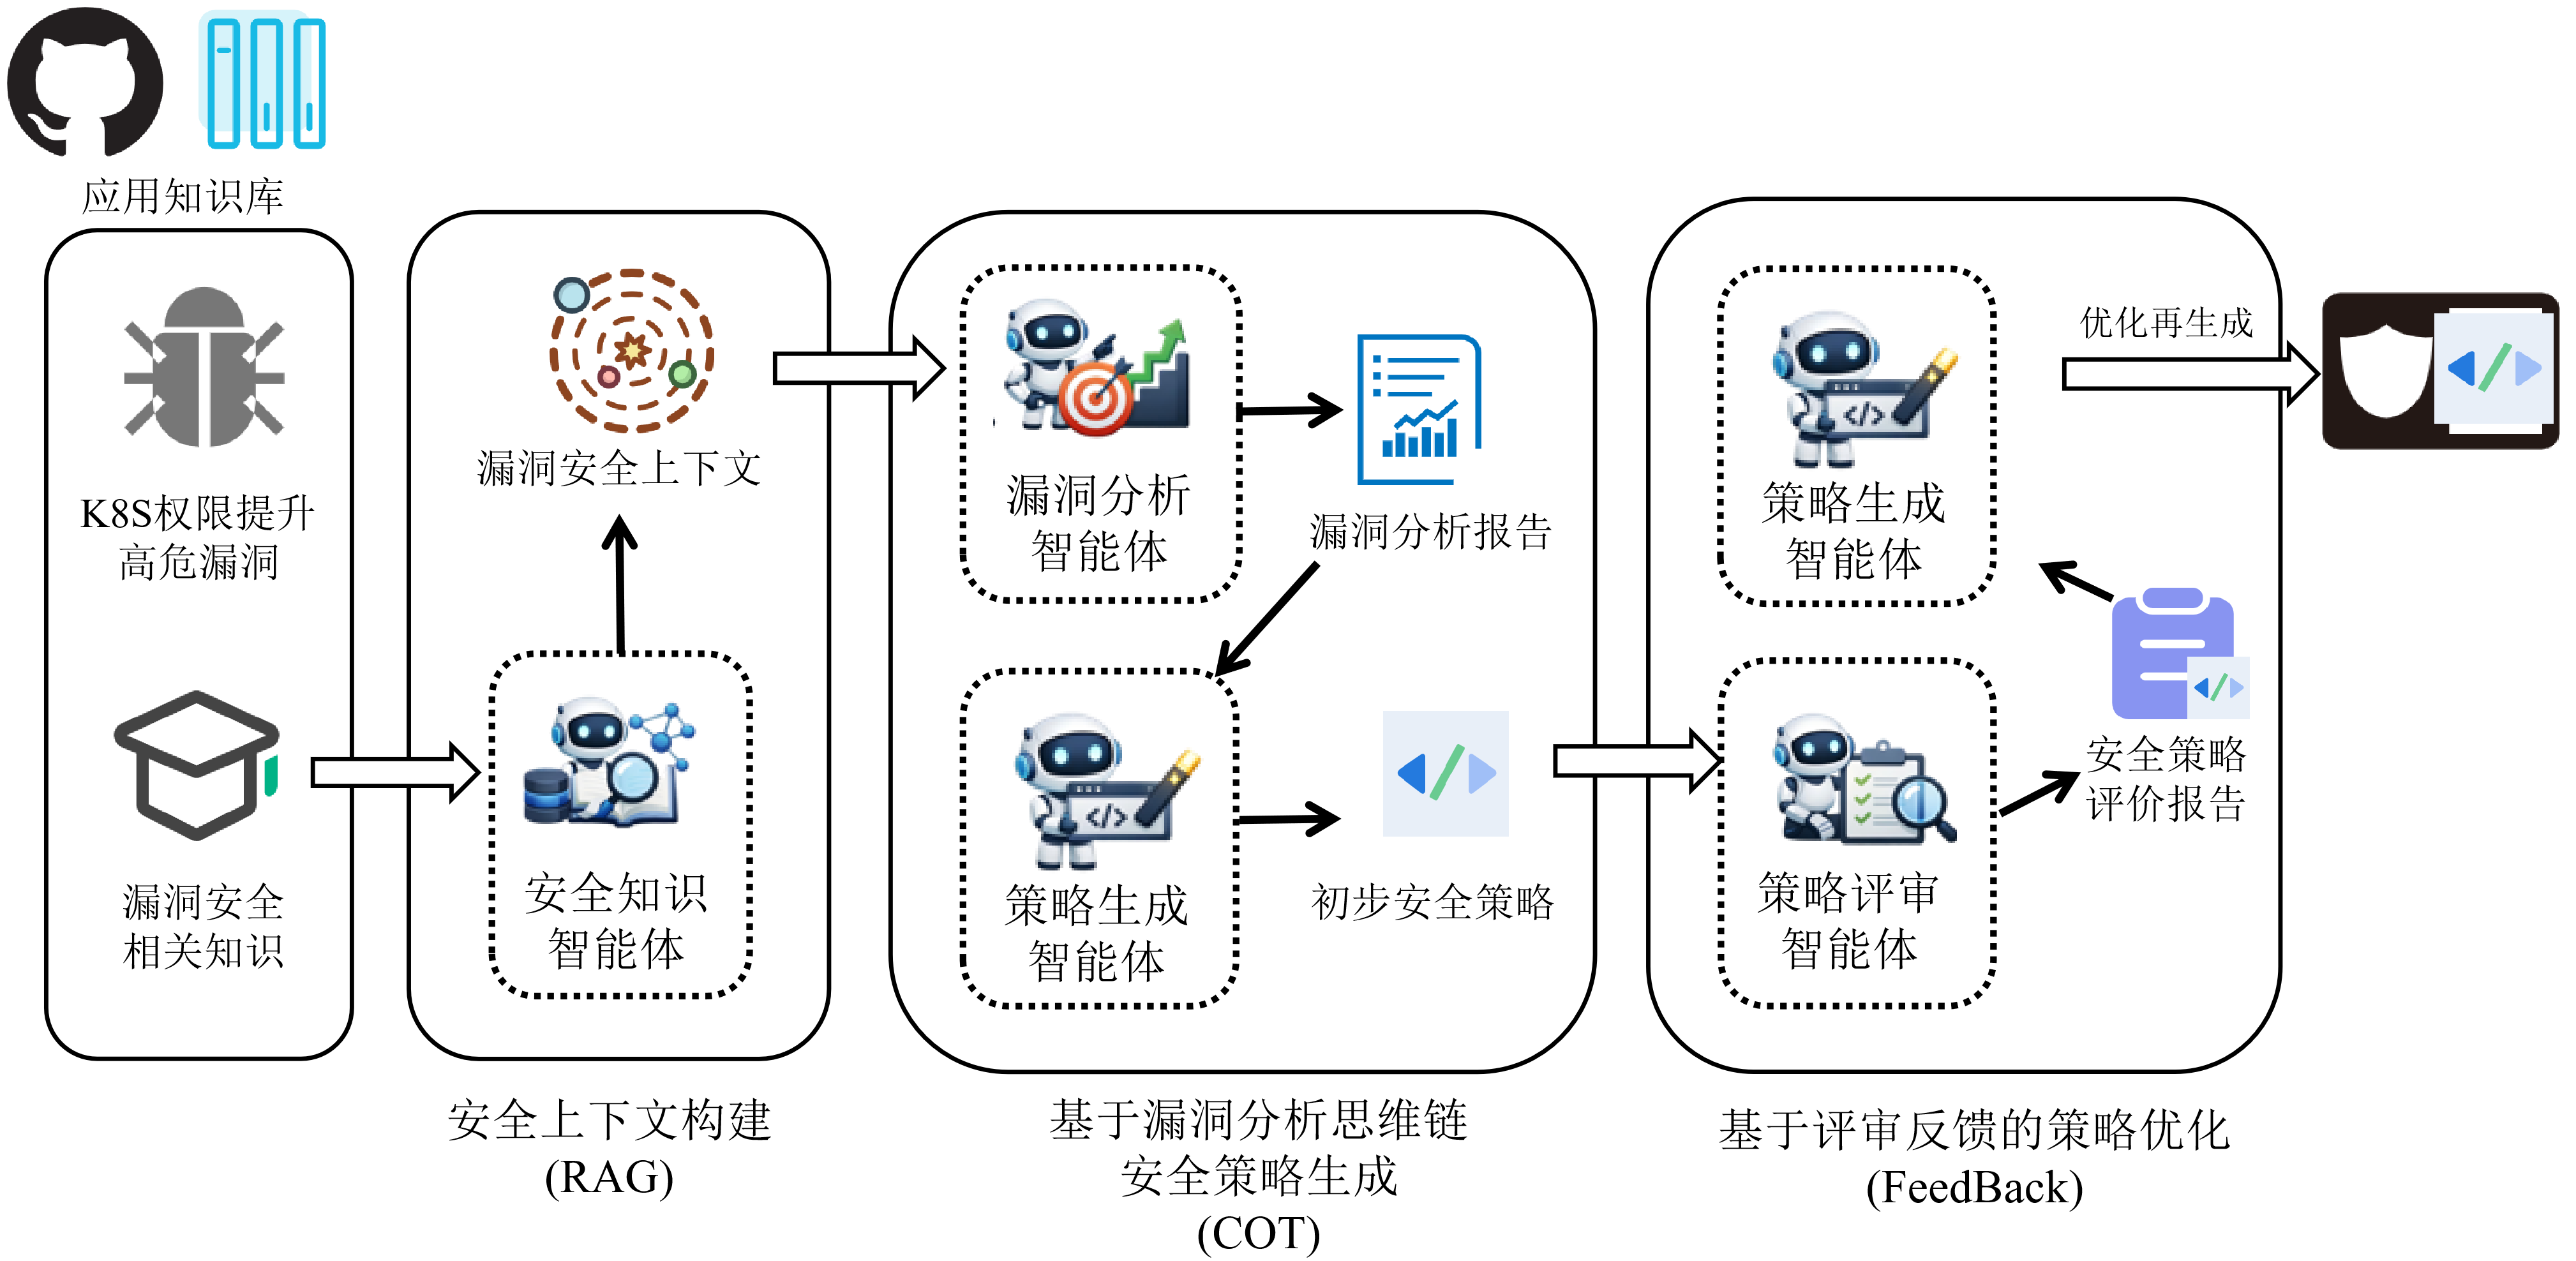
\includegraphics[width=1\textwidth]{images/method.png}
    \bicaption{多智能体协同的策略化漏洞防控工作流}{Multi-agent collaborative framework for strategy-based vulnerability prevention and control}\label{fig:method}
\end{figure}


\subsubsection{安全上下文构建}

安全上下文构建的关键在于保证证据可追溯。按照定义 2，证据集合记为 $c=\{\,\langle t_i,\mathit{src}_i\rangle\mid i\in[n_c] \,\}$。在知识库阶段，系统为每个片段记录来源元数据，如路径、URL、版本与位置；在生成阶段，再从知识库与安全材料中检索候选证据，并由\textbf{安全知识智能体}完成去重与提炼，输出触发条件、受影响组件、权限边界与可控点，同时保留对应的 $\mathit{src}_i$ 供复核。

为保证不同实验轮次中证据整理过程具有一致的输入输出边界，本文将该智能体的指令约束抽象为由角色、输入、任务和输出构成的四元模式，其在全流程中的统一定义见表~\ref{tab:agent-instruction-schema}。安全知识智能体的职责是将离散证据整理为带来源标识的结构化摘要，而不是直接给出策略建议。

\begin{PromptBox}{安全知识智能体提示词简化示例}
\begin{Verbatim}[breaklines,breakanywhere,mathescape=true]
你是云原生安全知识整理助手。
## 输入
漏洞实例 $v$ 与候选证据集合 $c$

## 任务
提炼受影响组件、触发条件、权限边界、攻击前提与缓解线索，
保留每条结论对应的来源标识。

## 输出
返回结构化证据摘要，不直接生成防控策略。
\end{Verbatim}
\end{PromptBox}

\subsubsection{基于漏洞分析思维链的策略生成}

本节将漏洞分析、技术选型与策略生成纳入统一的结构化约束，要求各环节输出可复核的中间结论。与仅给出自然语言建议相比，这种做法能够减少信息缺失与表述歧义。

首先，\textbf{漏洞分析智能体}基于漏洞摘要与安全上下文 $c$ 形成结构化分析结果，覆盖漏洞类型、攻击路径、影响范围与风险类别，并与前述成因分类体系保持一致。随后，\textbf{策略生成智能体}在结构化指令约束与分步推理引导下，根据分析结论选择控制手段并组织动作序列。具体而言，它会结合平台可用能力，在身份与权限收敛、网络隔离、运行时约束与准入控制等手段之间确定实施路径，并将其映射为最终策略对象；当证据不足以支持唯一结论时，则显式保留待补充信息与必要假设。为保持方法主线清晰，同时保证实验过程可复现，本文保留简化后的提示词示例，并以表~\ref{tab:agent-instruction-schema}概括各智能体的统一约束。

\begin{table}[htb]
    \centering
    \bicaption{多智能体指令约束摘要}{Summary of instruction constraints for the multi-agent workflow}\label{tab:agent-instruction-schema}
    \small
    \setlength{\tabcolsep}{3pt}
    \renewcommand{\arraystretch}{1.1}
    \begin{tabular}{>{\raggedright\arraybackslash}p{2.4cm} >{\raggedright\arraybackslash}p{3.0cm} >{\raggedright\arraybackslash}p{3.6cm} >{\raggedright\arraybackslash}p{4.0cm}}
        \toprule
        \textbf{智能体} & \textbf{输入} & \textbf{核心任务} & \textbf{输出约束} \\
        \midrule
        安全知识智能体 & 漏洞实例与候选证据片段 & 抽取受影响组件、触发条件、攻击前提、权限边界与缓解线索 & 输出带来源标识的结构化证据摘要 \\
        漏洞分析智能体 & 漏洞实例与安全上下文 & 形成漏洞类型、攻击路径、影响范围与风险类别的结构化分析 & 输出满足预定义模式的分析结果 \\
        策略生成智能体 & 中间分析结论、控制手段选择结果与安全上下文 & 生成监控或防护策略，并保持字段完整、一致且可验证 & 输出包含 \texttt{type}、\texttt{method} 与 \texttt{action} 的结构化策略对象 \\
        策略评审智能体 & 漏洞实例、候选策略集合与补充约束 & 从有效性、干扰风险与验证需求等方面形成评审意见 & 输出包含总体结论与逐策略点评的结构化评审结果 \\
        策略优化智能体 & 漏洞实例、候选策略集合与评审结论 & 吸收有效控制、剔除高噪声建议，并补齐前置条件与回滚边界 & 输出优化后策略及相对原候选的改进说明 \\
        评价智能体 & 匿名化与随机化后的同类型候选策略集合 & 在 $E$、$I$、$D$ 三个维度上给出严格排序 & 输出满足预定义模式的维度排序结果及必要判据 \\
        \bottomrule
    \end{tabular}
\end{table}

策略生成阶段需要在统一的数据模式下将分析结论映射为可部署的策略对象，因此除任务目标外，还需明确输出字段与约束边界。表~\ref{tab:agent-instruction-schema}中漏洞分析与策略生成两类智能体的约束，共同保证了这一映射过程的稳定性。

\begin{PromptBox}{漏洞分析智能体提示词简化示例}
\begin{Verbatim}[breaklines,breakanywhere,mathescape=true]
你是 Kubernetes 漏洞分析助手。
## 输入
漏洞实例 $v$ 与安全上下文 $c$

## 任务
给出漏洞类型、攻击路径、影响范围与成因分类，
并指出导致权限提升的关键环节。

## 输出
返回结构化分析结果；证据不足处显式标注 assumptions。
\end{Verbatim}
\end{PromptBox}

\begin{PromptBox}{策略生成智能体提示词简化示例}
\begin{Verbatim}[breaklines,breakanywhere,mathescape=true]
你是云原生安全策略生成助手。
## 输入
中间分析结论、可用控制手段与安全上下文 $c$

## 任务
围绕监控或防护目标生成策略 $\pi=\langle \mathit{type},\mathit{method},\mathit{action} \rangle$，
优先给出可部署、可验证、可回滚的措施。

## 输出
返回结构化策略对象；若信息不足，显式说明前置假设。
\end{Verbatim}
\end{PromptBox}

为与前述基本概念定义保持一致，策略对象统一采用 \texttt{type}、\texttt{method} 与 \texttt{action} 三字段模式。其中，\texttt{type} 用于区分监控型与防护型策略，\texttt{method} 用于描述控制机理，\texttt{action} 用于承载与之对应的可执行表达，如规则片段、配置约束或执行命令。当一项策略包含多条控制措施时，\texttt{method} 与 \texttt{action} 均表示为等长序列，并通过位置对应关系保持语义一致。


为保证候选策略具有可比性与交付价值，本文进一步要求其至少满足以下条件：覆盖明确的防控目标，包含可验证的实施步骤，并对潜在副作用与回滚边界作出清晰说明。

候选策略集合 $\Pi_v$ 通过多候选并行生成方式获得，即围绕同一漏洞构造多个结构化策略对象，以探索不同控制思路与实施路径。为避免异质目标混合比较，生成结果在进入评价阶段前按策略类型划分为 $\Pi_v^{\mathrm{mon}}$ 与 $\Pi_v^{\mathrm{prot}}$，并分别进入后续评价与排序环节。

在进入交付与评估阶段之前，系统还需对生成结果进行规范化整理，包括统一字段格式、补齐必要步骤、清理冗余信息，并在证据不足处显式标记假设条件与前置依赖。

\subsubsection{基于评审反馈的策略优化}

在候选策略生成之后，流程进入评审、反馈与再生成的迭代优化环节，以降低误报与运维噪声，提升可部署性与一致性。系统首先通过并行生成获得多份候选，形成 $\Pi_v$；随后由\textbf{策略评审智能体}给出结构化评审，包括有效点、风险、验证要点与缺失信息；最后由\textbf{策略优化智能体}合并可行措施、剔除不可行建议，并补齐前置条件与回滚方案。

为保证评审阶段具有一致的比较口径，本文将评审与优化两个环节的指令约束统一纳入表~\ref{tab:agent-instruction-schema}所示模式，并保留简化后的提示词示例，用以展示其输入边界、判断依据与输出结构。

策略优化阶段的目标是将多份候选与评审反馈压缩为单一、可交付的最终策略，因此其关键不在于模板表述本身，而在于前序评审信息的吸收边界、修订依据与回滚约束是否得到显式保留。

\begin{PromptBox}{策略评审智能体提示词简化示例}
\begin{Verbatim}[breaklines,breakanywhere,mathescape=true]
你是云原生安全策略评审助手。
## 输入
漏洞实例 $v$、候选策略集合 $\Pi_v$ 及补充约束

## 任务
从有效性、无干扰性与验证需求三个方面比较候选，
指出优势、风险与缺失信息。

## 输出
返回结构化评审结果，包含总体结论与逐策略点评。
\end{Verbatim}
\end{PromptBox}

\begin{PromptBox}{策略优化智能体提示词简化示例}
\begin{Verbatim}[breaklines,breakanywhere,mathescape=true]
你是云原生安全策略优化助手。
## 输入
漏洞实例 $v$、候选策略集合 $\Pi_v$ 与评审结论

## 任务
保留有效控制，删除高噪声或不可行措施，
补齐前置条件、验证步骤与回滚边界。

## 输出
返回优化后的最终策略，说明保留、删除与修订原因。
\end{Verbatim}
\end{PromptBox}

\subsubsection{基于排序的质量评价}
基于共识得分可得到维度 $\delta$ 的\textbf{共识排序} $\bar R_{\delta}$，即按 $\hat S_{\delta}(\pi)$ 从大到小进行排序。为保证输出为严格排序，若出现数值相等，则按预先约定的确定性规则打破平分，例如依次比较各评审主体的原始排名，并以匿名编号作为最终判别。

为刻画评审一致性与不确定性，可进一步定义分歧度量，例如秩的加权方差：
\[
U_{\delta}(\pi)=\sum_{h\in\mathcal{H}} w_h\cdot\big(r_{\delta}^{(h)}(\pi)-\bar r_{\delta}(\pi)\big)^2,
\quad \bar r_{\delta}(\pi)=\sum_{h\in\mathcal{H}} w_h\cdot r_{\delta}^{(h)}(\pi)
\]
当 $U_{\delta}(\pi)$ 较大时，表示该策略在该维度上存在明显分歧，需在后续决策中优先人工复核。

在获得三维共识质量后，进一步给出总体质量函数 $Q: \Pi_v^{\tau}\to[0,1]$：
\[
Q(\pi)=\alpha_E\hat S_E(\pi)+\alpha_I\hat S_I(\pi)+\alpha_D\hat S_D(\pi),\quad \alpha_E+\alpha_I+\alpha_D=1
\]
其中 $\alpha_E,\alpha_I,\alpha_D$ 是三个维度的权重，用于将有效性、无干扰性和可部署性的偏好映射到最终排序。该权重可按业务场景配置：例如在应急与临时缓解场景下可提高 $\alpha_E,\alpha_D$；在生产稳定性优先场景下可提高 $\alpha_I$。

在本文的安全防控语境下，若无额外业务约束，默认偏好应体现有效性优先，即 $\alpha_E>\alpha_I>\alpha_D$。例如可取 $\alpha_E=0.5,\alpha_I=0.3,\alpha_D=0.2$ 作为默认基线，具体数值可结合组织的风险偏好与运维能力进行微调。


为避免权重选择导致结论出现偶然变化，实验中可对 $\alpha$ 做简单敏感性分析，例如在合理范围内扰动 $\alpha$ 并观察总排名是否稳定，再将不稳定样本优先交由专家复核。对任一固定类型 $\tau$，最终总排名 $\bar R^{\tau}$ 由 $Q(\pi)$ 从大到小排序得到；为保证输出为严格排序，若出现 $Q(\pi)$ 相等，则按 $(\hat S_E,\hat S_I,\hat S_D)$ 的词典序进行细化，并在仍无法区分时以匿名编号作为最终判别。由此，系统可分别得到监控型与防护型候选的可审计交付结论。

\section{方法示例}

为更直观地说明上述方法在真实场景中的运行方式，下面以案例分析中的第一个漏洞 \mbox{CVE{-}2022{-}24768} 为例进行说明。该漏洞出现在 Argo CD 中，属于访问控制缺陷引发的权限提升问题。攻击者并不是直接突破 Kubernetes 的原生权限边界，而是先以普通 Argo CD 用户身份获得对特定 Application 的 \texttt{sync} 与 \texttt{override} 能力，或对其源代码仓库具备推送权限，再借助 GitOps 同步机制诱导控制平面创建超出其原始权限范围的高权限资源。对于这一类漏洞，方法首先接收 CVE 描述、组件版本、受影响对象和补丁信息等基础输入，并据此确定后续检索与分析的范围。下面结合证据归并、策略形成与后续修订过程，说明该方法在具体漏洞场景中的展开方式。

在安全上下文构建阶段，系统围绕该漏洞从公告说明、修复提交、Issue/PR 讨论、Argo CD 权限模型文档以及相关代码配置中检索证据片段，重点收集攻击前提、可被滥用的控制点、涉及的资源对象和已知缓解建议，并将这些内容整理为带来源标识的安全上下文。经归并后，与该漏洞直接相关的事实主要包括以下几个方面：

\noindent\textbf{相关证据可归纳为}
\begin{itemize}
    \item \textbf{受影响对象}：Argo CD 及其与 \texttt{Application}、\texttt{AppProject} 相关的控制平面能力；
    \item \textbf{前置条件}：攻击者拥有某个 \texttt{Application} 的 \texttt{sync+override} 权限，或对其源 Git/Helm 仓库具有 \texttt{push} 权限；
    \item \textbf{关键资产与控制点}：\texttt{AppProject} 中 \texttt{roles/policies} 的配置表达、\texttt{argocd-rbac-cm} 中的默认角色与高风险能力授权，以及集群内新增的高权限 \texttt{RoleBinding}/\texttt{ClusterRoleBinding}；
    \item \textbf{攻击链}：低权身份影响期望状态，Argo CD 控制平面执行同步，随后创建高权限 RBAC 绑定并放大攻击者权限；
    \item \textbf{缓解线索}：收敛 \texttt{AppProject} 的创建更新权限，将默认能力压缩为只读，并对 \texttt{AppProject} 策略表达施加准入校验；
    \item \textbf{来源依据}：漏洞公告与版本说明、修复提交、Argo CD 官方 RBAC 与 \texttt{AppProject} 文档。
\end{itemize}

基于这些证据，可进一步归纳出该漏洞的核心并不在于容器逃逸或底层组件失陷，而在于低权用户能够借助 Argo CD 控制平面的高权限身份放大自身能力；其关键利用链包括获得应用同步影响能力、提交恶意资源清单、触发控制平面执行以及最终生成高权限 RBAC 绑定。通过这一分析，原本较为抽象的漏洞描述便可收敛为若干明确的控制点，例如限制 \texttt{AppProject} 与高风险资源的写入范围、收紧 \texttt{override} 等高危能力，以及补充对异常同步行为和权限变更的观测。

在此基础上，策略生成阶段围绕同一漏洞并行形成监控与防护两类候选策略。初步形成的方案通常已经能够覆盖主要风险，但在控制粒度、约束完整性和部署说明方面仍可能存在不足。以防护策略为例，早期形成的方案首先聚焦于 Argo CD RBAC 加固，其核心意图是将默认能力压缩到只读，并先行切断 \texttt{exec} 等高风险操作。其重点包括以下几个方面：

\noindent\textbf{防护方案的初步配置重点}
\begin{itemize}
    \item 优先给出 \texttt{argocd-rbac-cm} 的收敛方案，将 \texttt{policy.default} 设为 \texttt{role:readonly}，并保留 \texttt{applications}、\texttt{repositories}、\texttt{projects}、\texttt{clusters} 的只读能力；
    \item 代码中的关键收敛项包括 \texttt{p, role:readonly, applications, get, *, allow} 与 \texttt{p, role:readonly, exec, *, *, deny}；
    \item 该方案已经能够压缩默认授权面，但尚未覆盖 \texttt{AppProject} 中策略表达被滥用的问题，因此仍需结合后续评审进一步补全。
\end{itemize}

相应的配置片段可写为：

{\small
\begin{quote}
\verb|policy.default: role:readonly|\\
\verb|p, role:readonly, applications, get, *, allow|\\
\verb|p, role:readonly, exec, *, *, deny|
\end{quote}
}

上述方案已经体现出最小权限原则，但仍需检验其是否真正覆盖该漏洞的主要利用链。对于 \mbox{CVE{-}2022{-}24768} 而言，若某一候选仅提出升级版本或笼统地“加强 RBAC”，而没有具体约束 \texttt{sync}、\texttt{override}、\texttt{AppProject} 写入和高权限绑定创建等关键环节，则会在有效性维度上处于劣势；若某一方案直接禁止所有同步行为，则虽然拦截强度较高，但会因业务干扰过大而在无干扰性维度上失分。基于这一判断，前述方案中“只收敛默认角色、尚未限制 \texttt{AppProject} 策略表达”的缺口便显现出来，因此后续修订进一步补入了对 \texttt{AppProject} 规则的校验约束，例如禁止全局通配符放权、强制项目域前缀，并限制对全局高危资源的写权限。

\noindent\textbf{进一步补入的约束配置}
\begin{itemize}
    \item 在保留 RBAC 收敛思路的基础上，补入 Gatekeeper 准入控制模板，用于约束 \texttt{AppProject} 中的策略表达；
    \item 补充后的核心规则包括：禁止全局通配符放权，要求 subject 落在 \texttt{proj:<project>:<role>} 范围内，并禁止对 \texttt{projects}、\texttt{repositories}、\texttt{clusters}、\texttt{exec} 等高危资源授予写权限；
    \item 经过这一补充，原先遗漏的关键控制点被落实为可部署的准入规则，利用链上的防护缺口也随之收紧。
\end{itemize}

相应的 Gatekeeper 入口配置示例如下：

{\small
\begin{quote}
\verb|kind: K8sArgoCDAppProjectPolicies|\\
\verb|name: restrict-argocd-appproject-policies|\\
\verb|enforceProjPrefix: true|
\end{quote}
}

在此基础上，再对保留下来的方案从有效性、无干扰性与可部署性三个维度进行比较，并形成监控策略与防护策略的排序结果。对于该漏洞，更优的方案通常不是简单地“一刀切”禁用同步，也不是只保留原则性建议，而是将 Kubernetes RBAC 收敛、Argo CD 默认只读、准入控制校验与必要的审计观测组合起来，形成能够在补丁窗口期内实际落地的临时处置方案。由此可见，面向具体漏洞的临时防控并非依赖单一控制措施，而是需要经过证据整理、漏洞分析、方案形成与后续修订，最终得到可复核、可部署的结果。完整策略清单与案例部署细节见附录~\ref{app:cve-2022-24768} 和第六章案例分析。

\section{小结}
本章围绕云原生权限提升漏洞的防控需求，给出了从知识组织、候选生成到多评审聚合的完整方法链条。具体而言，本文统一定义了漏洞实例、安全上下文、策略对象与评价过程，构建了面向开源应用漏洞的可追溯知识库，并基于多智能体协同完成策略生成、评审与优化，最终通过三维评价与多源排名聚合模型实现对候选策略的可审计选择。上述设计为下一章的系统设计与实现以及后续实验验证奠定了方法基础。
